\section{连续釜式反应器的串联与并联}


\begin{frame}
    \frametitle{多釜串联的全混流反应器}

    由于反应器出口处反应物浓度最低，故全混流反应器总是在最低的反应物浓度下操作，很多情况下将会影响反应的效率。为了利用全混流反应器的混合均匀、温度易控的优点，又使反应不全部在反应物浓度最低的条件下进行，工业上经常将全混流反应器串联起来使用，称为多釜串联的全混流反应器(CSTRs in series)。

    \centering 
    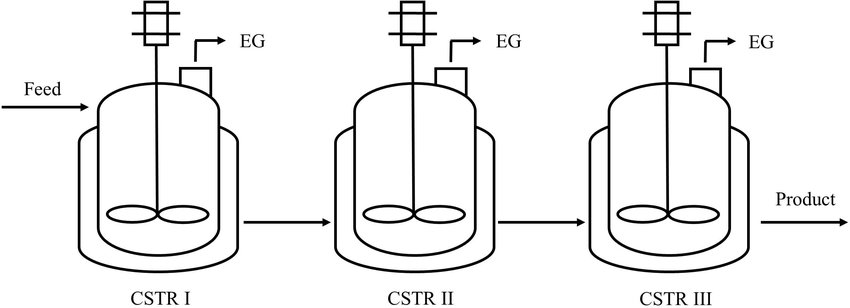
\includegraphics[height=4cm]{figs/CSTRs-in-series.png}

\end{frame}


\begin{frame}
    \frametitle{连续釜式反应器反应体积的几何图示}

    连续釜式反应器反应体积$V_{\mathrm{r}}=\frac{Q_{0} c_{\mathrm{A} 0} X_{\mathrm{A}}}{-\mathscr{R}_{\mathrm{A}}}$，以$X_{\mathrm{A}}$对$\frac{1}{-\mathscr{R}_{\mathrm{A}}}$作图，
    \begin{center}
        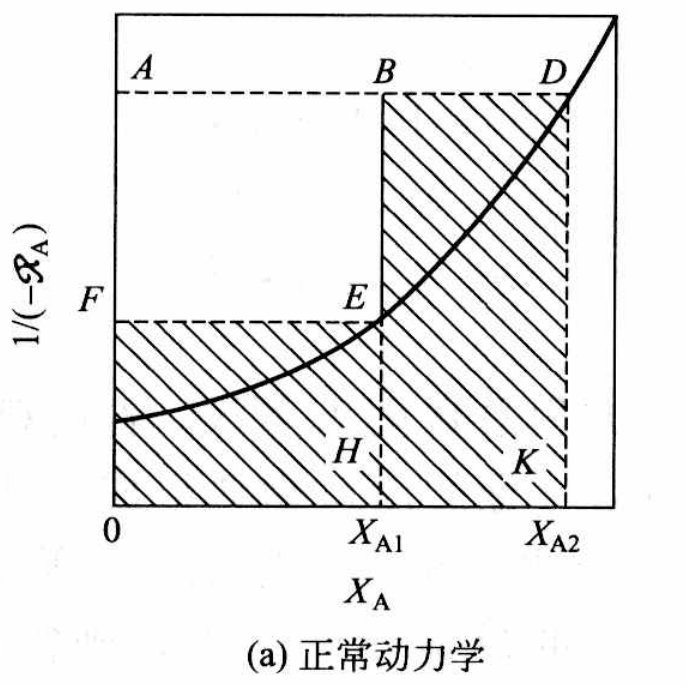
\includegraphics[width=0.8\linewidth]{figs/fig3.4.png}
    \end{center}
    

\end{frame}


\begin{frame}
    \frametitle{多釜并联}

    \begin{columns}[c]
        \column{5cm}
            \\~
            \\~
            \\
            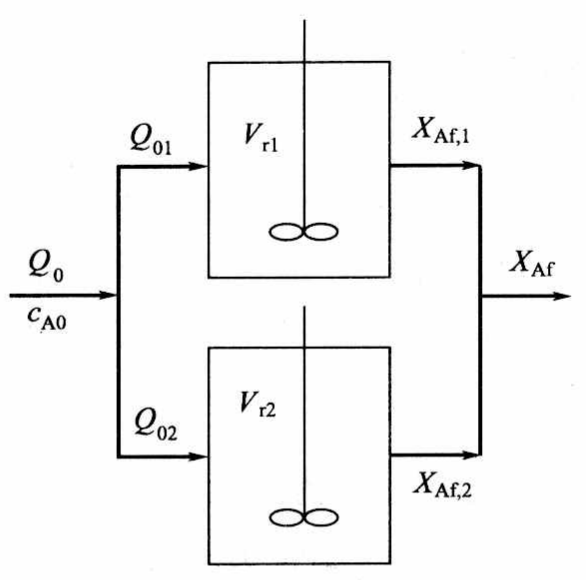
\includegraphics[width=\linewidth]{figs/fig3.5.png}
        \column{8.5cm}
            \begin{itemize}
                \item[\bullet] 当用单釜进行反应所需的反应体积过大而难以加工制造时，就需用若干个体积较小的反应釜。
                \item[\bullet] 具有正常动力学的反应应采用串联方式，若为反常动力学，则应各釜单独操作，即采用并联方式。
                \item[\bullet] 各釜的进料量分配原则是保证各釜的空时相同，也就是说各釜的出口转化率相等，这样效果最佳。即各釜的进料量与各釜的反应体积成正比。
            \end{itemize}            
    \end{columns}

\end{frame}


\begin{frame}
    \frametitle{串联釜式反应器的计算}

    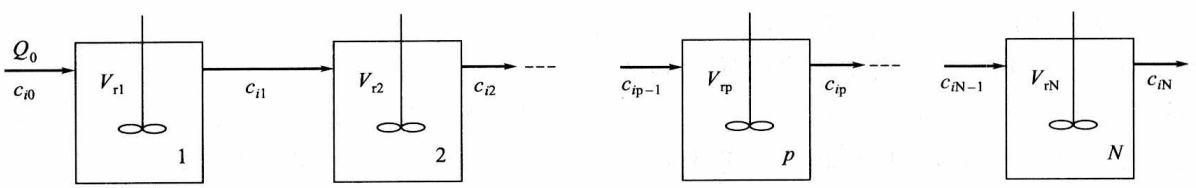
\includegraphics[width=\linewidth]{figs/fig3.6.png}

    由$N$个反应体积分布为，$V_\mathrm{r1}$，$V_\mathrm{r2}$，$\cdots$，$V_{\mathrm{r}N}$的釜组成的串联釜式反应器。若求最终转化率或收率，对各釜分别作关键组分$i$的物料衡算得下列方程组
    \[
        V_{\mathrm{rp}}=\frac{Q_{0}(c_{i \mathrm{p}}-c_{i \mathrm{p}-1})}{-\mathcal{R}_{i\mathrm{p}}} \qquad\left[\begin{array}{l}
        p=1,2, \cdots, N \\
        i=1,2, \cdots, K 
        \end{array}\right]
    \]

    计算从第1釜开始，由于该釜的进口组成已知，可求出口组成，这也就是第2釜的进口组成。依此类推，直至第N釜即为所求。这种算法称为逐釜计算法。

\end{frame}


\begin{frame}
    \frametitle{串联釜式反应器的计算}

    \large 实际设计中往往是已知进料量和组成，确定达到规定的输出物料组成时所需的釜数和各釜的反应体积。
    
    一般情况下，釜数越多，总反应体积越小，从这点看，多用几个釜串联操作是有利的。但是，釜数多了，相应地管道阀门和控制仪表等也要增多，操作的复杂程度也随之增加，所以，应根据具体情况从经济的角度出发确定最佳的釜数。此外，各釜的操作温度及浓度的确定，即各釜的反应体积间的比例是一个优化问题。一般把各釜做成相同的大小，是从机械加工制造方便的角度出发的。

\end{frame}


\begin{frame}
    \frametitle{串联釜式反应器的计算(一级单一反应)}

    以一级单一反应为例，以反应物A为关键组分
    \[
        V_{\mathrm{rp}}=\frac{Q_{0}(c_{\mathrm{Ap}-1}-c_{\mathrm{Ap}})}{(-\mathscr{R}_{\mathrm{Ap}})} =\frac{Q_{0} c_{\mathrm{A} 0}(X_{\mathrm{Ap}}-X_{\mathrm{Ap}-1})}{-\mathscr{R}_{\mathrm{Ap}}(X_{\mathrm{Ap}})} =\frac{Q_{0}(X_{\mathrm{Ap}}-X_{\mathrm{Ap}-1})}{k(1-X_{\mathrm{Ap}})}
    \]

    假定各釜反应体积相等，则各釜的空时相等，设为$\tau$；各釜温度相同，反应速率常数均为$k$。则上式可变为
    \[
        \frac{1-X_{\mathrm{Ap}-1}}{1-X_{\mathrm{Ap}}}=1+k \tau \qquad (p=1,2,\cdots , N)
    \]

    将这$N$个方程相乘则有
    \[
        \frac{1}{1-X_{\mathrm{AN}}}=(1+k \tau)^{N} \quad \text{或} \quad \tau=\frac{1}{k}\left[\left(\frac{1}{1-X_{\mathrm{AN}}}\right)^{1 / N}-1\right]
    \]

\end{frame}


\begin{frame}
    \frametitle{作图法求串联釜式反应器出口转化率}

    \begin{columns}[c]
        \column{5cm}
            \\~
            \\~
            \\    
            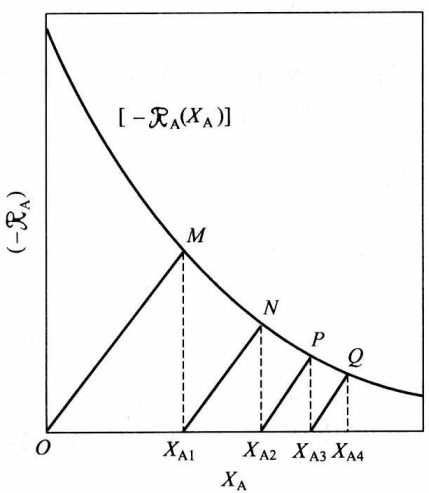
\includegraphics[width=\linewidth]{figs/fig3.7.png}
        \column{8.5cm}
            对于非一级反应，需要逐釜计算。

            将$V_{\mathrm{rp}}=\frac{Q_{0} c_{\mathrm{A} 0}(X_{\mathrm{Ap}}-X_{\mathrm{Ap}-1})}{-\mathscr{R}_{\mathrm{Ap}}(X_{\mathrm{Ap}})}$改写成
            \[
                -\mathscr{R}_{\mathrm{A}}=\frac{c_{\mathrm{A} 0}}{\tau_{\mathrm{p}}} X_{\mathrm{Ap}}-\frac{c_{\mathrm{A} 0}}{\tau_{\mathrm{p}}} X_{\mathrm{Ap}-1}
            \]

            在$X_\mathrm{A}$-$(-\mathcal{R}_\mathrm{A})$图上，物料衡算式为一直线，其斜率为$c_{\mathrm{A} 0} / \tau_{\mathrm{p}}$。
            
            各釜温度相图，所以只需根据反应速率方程绘制一条动力学曲线。因为出口转化率既要满足反应速率方程，又要符合物料衡算式，所以可由两者交点决定釜的出口状态。
    \end{columns}

\end{frame}


\begin{frame}[t]{}
    \begin{example}
        采用双釜串联的连续釜式反应器，等温下进行某均相反应\ce{A -> B}，$r_\mathrm{A}=5.2c_\mathrm{A}$ (\si{mol.L^{-1}.h^{-1}})，每天生产B 20kmol，A的初始浓度为2mol/L，最终转化率为80\%。计算总反应体积。
    \end{example}\pause

    \[
        \tau=\frac{1}{5.2}\left[\left(\frac{1}{1-0.8}\right)^{1 / 2}-1\right]=0.2377 \mathrm{h}
    \]

    \[
        V_\mathrm{r}=2Q_0 \tau = 2 \times 520.8 \times 0.2377 = 247.59 \mathrm{L}
    \]

\end{frame}


\begin{frame}
    \frametitle{串联釜式反应器各釜最佳反应体积比}

    釜数及最终转化率已规定的情况下，为了使总的反应体积最小，各釜的反应体积存在一最佳的比例。现设所进行的为单一反应，则总反应体积
    \[
        V_{\mathrm{r}}=V_{\mathrm{r} 1}+\cdots+V_{\mathrm{rN}}=Q_{0} c_{\mathrm{A} 0}\left[\frac{X_{\mathrm{A} 1}-X_{\mathrm{A} 0}}{\left(-\mathscr{R}_{\mathrm{A} 1}\right)}+\frac{X_{\mathrm{A} 2}-X_{\mathrm{A} 1}}{\left(-\mathscr{R}_{\mathrm{A} 2}\right)}+\cdots+\frac{X_{\mathrm{AN}}-X_{\mathrm{AN}-1}}{\left(-\mathscr{R}_{\mathrm{AN}}\right)}\right]
    \]

    将上式分别对$X_\mathrm{Ap}$求导得
    \[
        \frac{\partial V_{\mathrm{r}}}{\partial X_{\mathrm{Ap}}}=Q_{0} c_{\mathrm{A} 0}\left[\frac{1}{\left(-\mathscr{R}_{\mathrm{Ap}}\right)}-\frac{1}{\left(-\mathscr{R}_{\mathrm{Ap}+1}\right)}+\left(X_{\mathrm{Ap}}-X_{\mathrm{Ap}-1}\right) \frac{\partial \frac{1}{\left(-\mathscr{R}_{\mathrm{Ap}}\right)}}{\partial X_{\mathrm{Ap}}}\right]
    \]
    令${\partial V_{\mathrm{r}}}/{\partial X_{\mathrm{Ap}}}=0$有$\frac{1}{\left(-\mathscr{R}_{\mathrm{Ap}+1}\right)}-\frac{1}{\left(-\mathscr{R}_{\mathrm{Ap}}\right)}=\left(X_{\mathrm{Ap}}-X_{\mathrm{Ap}-1}\right) \frac{\partial \frac{1}{\left(-\mathscr{R}_{\mathrm{Ap}}\right)}}{\partial X_{\mathrm{Ap}}}$
    
    这就是保证总反应体积最小所必须遵循的条件。解方程式组可得$X_{\mathrm{Ap}}$和$V_{\mathrm{rp}}$。
    
\end{frame}


\begin{frame}
    \frametitle{串联釜式反应器各釜最佳反应体积比}

    进行一级不可逆反应时，
    \[
        \frac{X_{\mathrm{Ap}+1}-X_{\mathrm{Ap}}}{1-X_{\mathrm{Ap}+1}}=\frac{X_{\mathrm{Ap}}-X_{\mathrm{Ap}-1}}{1-X_{\mathrm{Ap}}}
    \]
    上式可改写成
    \[
        \frac{Q_{0} c_{\mathrm{A} 0}(X_{\mathrm{Ap}+1}-X_{\mathrm{Ap}})}{k c_{\mathrm{A} 0}(1-X_{\mathrm{Ap}+1})}=\frac{Q_{0} c_{\mathrm{A} 0}(X_{\mathrm{Ap}}-X_{\mathrm{Ap}-1})}{k c_{\mathrm{A} 0}(1-X_{\mathrm{Ap}})}
    \]
    即\[V_{\mathrm{rp}+1}=V_{\mathrm{rp}}\]

    由此可见，串联釜式反应器进行一级不可逆反应时，各釜的反应体积相等时，总反应体积最小。

\end{frame}


\begin{frame}
    \frametitle{串联釜式反应器各釜最佳反应体积比}

    用串联釜式反应器进行$\alpha$ 级反应时，最佳反应体积：
    \begin{itemize}
        \item[1] $\alpha=1$时，各釜体积相等
        \item[2] $\alpha>1$时，小釜在前，大釜在后
        \item[3] $\alpha<1$时，大釜在前，小釜在后
        \item[4] $\alpha=0$时，反应速率与浓度无关，无论多少釜串联，与单釜反应体积相等
        \item[5] $\alpha<0$时，单釜操作优于串联操作
    \end{itemize}

\end{frame}


\begin{frame}[t]{}
    \begin{example}
        以硫酸为催化剂，由醋酸和丁醇反应可制得醋酸丁酯。仓库里闲置着两台反应釜，一台的反应体积为\SI{3}{m^3}，另一台则为\SI{1}{m^3}。现拟将它们用来生产醋酸丁酯，初步决定采用等温连续操作，原料中醋酸的浓度为\SI{0.15}{kmol.m^3}，丁醇则大量过剩，该反应对醋酸为2级，在反应温度下反应速率常数为\SI{1.2}{L.mol^{-1}.h^{-1}}，要求醋酸的最终转化率不小于50\%。
        
        (1) 你认为采用怎样的连接方式醋酸丁酯的产量最大？为什么？试计算你所选用的方案得到的醋酸丁酯产量。
        
        (2) 如果进行的反应是一级反应，这两台反应器的串联方式又应如何？

        (3)如果进行的反应是一级反应，并更换为两台反应体积均为\SI{2}{m^3}的反应器串联，醋酸丁酯产量是多少？
    \end{example}

\end{frame}